\documentclass[11pt]{article}
\usepackage{fullpage}
\usepackage{graphicx}
\author{Thierry Matthey\\{\tt matthey@ii.uib.no}}

\title{Performance of \textsc{ProtoMol}}

\begin{document}
\maketitle
\begin{abstract}
A collection of performance tests of {\sc ProtoMol} during its development
and a note about how to tune the performance of force algorithms.
\end{abstract}




\section{Performance: \textsc{ProtoMol} 1.8.3 vs. \textsc{ProtoMol} 2.0.2 }
\begin{table}[htb]
\small
  \begin{center}
    \begin{tabular}{|c|p{1.7cm}|l|l|l|l|l|l|l|l|}\hline
Ver. & \multicolumn{2}{|l|}{Machine}  & Compiler & \multicolumn{3}{|c|}{Vacuum} & \multicolumn{3}{|c|}{PBC} \\\hline
 \multicolumn{4}{|c|}{}  & \multicolumn{6}{|c|}{Cell Size} \\\hline
 \multicolumn{4}{|c|}{} & 10 & 5 & 3$\frac{1}{3}$  & 10 & 5 & 3$\frac{1}{3}$ \\\hline
2.0.2 & Dual AMD Opteron & lcsl & gcc 3.2.3 &  47.77 &  38.37 &  42.65 &  83.50&  57.51 &  61.98  \\\hline
1.8.3 & Dual AMD Opteron & lcsl & gcc 3.2.3 &  49.66 &  41.72 &  46.73 &  99.05&  74.47 &  95.90  \\\hline
2.0.2 & Dual AMD Opteron & lcsl & gcc 3.2.3 & 341.98 & 274.11 & 303.87 & 645.56& 417.45 & 428.67 \\\hline
1.8.3 & Dual AMD Opteron & lcsl & gcc 3.2.3 & 350.59 & 296.86 & 329.28 & 848.47& 555.22 & 665.11 \\\hline


    \end{tabular}
  \end{center}
  \caption{BProtoMol 1.8.3 vs 2.0.2: BPTI 14281 Atoms / ApoA1 92224 Atoms, 100 Steps.}
\end{table}

\clearpage

\section{Performance: \textsc{ProtoMol} 1.8.3}

\begin{table}[htb]
\small
  \begin{center}
    \begin{tabular}{|p{1.7cm}|l|l|l|l|l|l|l|l|}\hline
\multicolumn{2}{|l|}{Machine}  & Compiler & \multicolumn{3}{|c|}{Vacuum} & \multicolumn{3}{|c|}{PBC} \\\hline
 \multicolumn{3}{|c|}{}  & \multicolumn{6}{|c|}{Cell Size} \\\hline
 \multicolumn{3}{|c|}{} & 10 & 5 & 3$\frac{1}{3}$ & 10 & 5 & 3$\frac{1}{3}$\\\hline
Dual AMD Opteron 248 2.2GHz & le04 & Intel 8.0 & 57.6068 & 46.53375 & 46.78541 & 104.51191 & 75.19006 & 84.90123\\\hline
Dual AMD Opteron 248 2.2GHz & le04 & gcc 3.2.2 & 42.23086 & 34.98725 & 36.11871 & 78.57884 & 61.0053 & 69.73622\\\hline
Pentium(R) 4 2.53GHz & romhegg & Intel 8.0 & 82.61629 & 64.27086 & 63.91178 & 131.30994 & 93.24453 & 103.0066\\\hline
Pentium(R) 4 2.53GHz & romhegg & gcc 3.2.2 & 113.0993 & 94.08331 & 86.44412 & 182.61486 & 134.46937 & 146.3645\\\hline
P4+ v2.2 1.6GHz (*) & blade & xlC 6 &  &  &  &  &  & \\\hline
P4+ v2.2 1.6GHz & blade & gcc 3.2.3 & 114.22825 & 98.49399 & 98.75213 & 172.38679 & 135.47089 & 145.3059\\\hline
P4 1.3Ghz & tre & xlC 6 & 124.77146 & 104.73123 & 108.48935 & 199.67187 & 153.70434 & 170.16276\\\hline
Dual AMD Opteron 2.0Ghz (*) & c0-0 & pathCC 1.2 &  &  &  &  &  & \\\hline
Dual AMD Opteron 2.0Ghz & c0-0 & gcc 3.2.3 & 50.73854 & 42.55911 & 43.812 & 96.66381 & 73.69411 & 82.10057\\\hline
MIPS R14000 1.4 & gridur & MIPSpro 7.4 & 126.04032 & 106.59266 & 118.52494 & 198.53973 & 163.74625 & 196.26711\\\hline
    \end{tabular}
  \end{center}
  \caption{BProtoMol 1.8.3: BPTI 14281 Atoms, 100 Steps.}
\end{table}

\clearpage

\section{Performance: \textsc{ProtoMol} 2000.03.10 vs. \textsc{NAMD 2.2}}
Runs were performed on a SGI Onyx2 (250MHz r10000). The times represent the
wall time [s] for 10 steps, sequential. For every step \textsc{ProtoMol} uses plain
Ewald summation, where \textsc{NAMD2} uses PME. 

\subsection{ApoA1, 92224 atoms}
\begin{table}[htb]
  \begin{center}
    \begin{tabular}{|c|r||c|r|}\hline
      \multicolumn{2}{|c||}{\textsc{ProtoMol}}&\multicolumn{2}{c|}{ \textsc{NAMD2}}\\\hline\hline
      \multicolumn{4}{|c|}{Periodic boundary conditions}\\\hline
      Plain Ewald         & 2152.45& PME                 &  712.96\\\hline
      Cutoff              &  407.94& Cutoff              & 277.45\\\hline\hline
      \multicolumn{4}{|c|}{Normal boundary conditions}\\\hline
      Cutoff              &  304.86& Cutoff              & 220.87\\\hline
      Full Coulomb        &18662.70& Full Coulomb        &--  \\\hline
      Full Coulomb \& VdW & -- & Full Coulomb \& VdW & -- \\\hline
    \end{tabular}
  \end{center}
  \caption{ApoA1, 92224 atoms, cutoff of 12A.\label{ApoA192224}}
\end{table}

\subsection{BPTI, 14281 atoms}
\begin{table}[htb]
  \begin{center}
    \begin{tabular}{|c|r||c|r|}\hline
      \multicolumn{2}{|c||}{\textsc{ProtoMol}}&\multicolumn{2}{c|}{ \textsc{NAMD2}}\\\hline\hline
      \multicolumn{4}{|c|}{Periodic boundary conditions}\\\hline
      Plain Ewald         & 209.38& PME                 &  57.10\\\hline
      Cutoff              &  33.19& Cutoff              &  22.53\\\hline\hline
      \multicolumn{4}{|c|}{Normal boundary conditions}\\\hline
      Cutoff              &  25.36& Cutoff              &  20.00\\\hline
      Full Coulomb        & 455.03& Full Coulomb        & --\\\hline
      Full Coulomb \& VdW & 349.43& Full Coulomb \& VdW & 351.49\\\hline
    \end{tabular}
  \end{center}
  \caption{BPTI, 14281 atoms, cutoff of 10A.\label{BPTI14281}}
\end{table}

\clearpage
\section{Tuning \sc{ProtoMol}}

Since {\sc ProtoMol} provides wide variety of different force
algorithms, which can be combined arbitrary, it may not always be simple to
find the an appropriate parametrization and force definition.

\subsection{Direct methods}

For the direct methods --  all pair-wise interactions are considered
-- on may change the \texttt{blocksize} in order to tweak the block size of
the sub matrices and improve the cache hits. The direct methods do compute sub matrix by sub
matrix and do not depend an the cell list algorithms, i.e.,
\texttt{cellsize} has no influence. Note that changing the block size does change the
order of computing the interactions, e.g., is the block size $> N$
(number of atoms), the algorithms does a simple 2-nested loop over all
atoms. 
 

\subsection{Cutoff methods}

The cutoff methods use the cell list algorithm (see
Fig.\ref{fig:cellalg}) in order to retrieve all
neighbor particles in $O(N)$. The Cell list algorithm requires a
cell. The algorithm keeps track of all particles residing in the cell
and can therefore retrieve them in $O(N)$. It finds all neighbors
\begin{figure}[hb]
\centerline{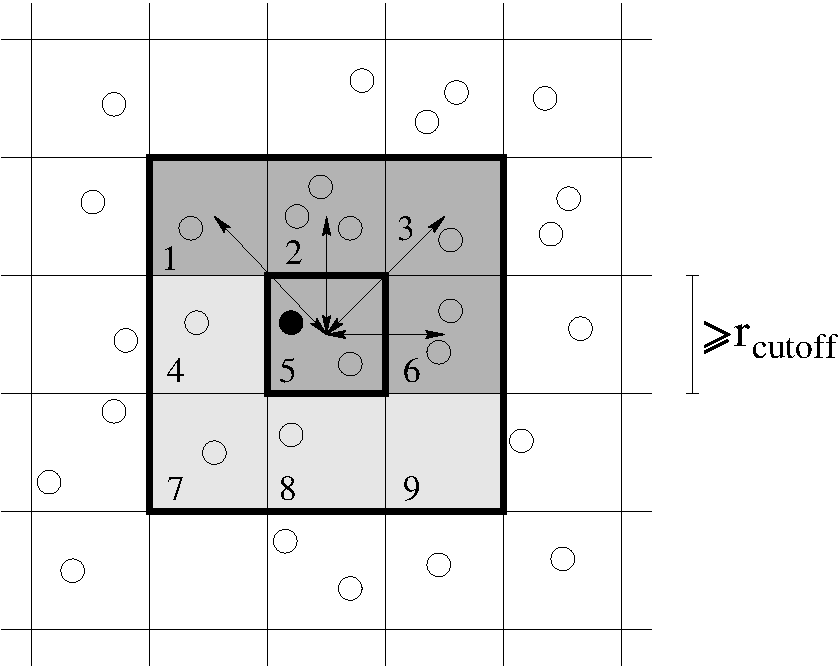
\includegraphics[width=7cm]{cell_algo_cell.pdf}}
\caption{Partition of cells, where cell no. 5 is the
    origin and 1-4, 6-9 the neighbor cells. Cell no. 6, 3, 2 and 1
    describe the interaction path.}
\label{fig:cellalg}
\end{figure}
(candidates) of all particles of the original cell, which defines the minimal dimension of a single
\begin{figure}[hbt]
\centerline{\rotatebox{-90}{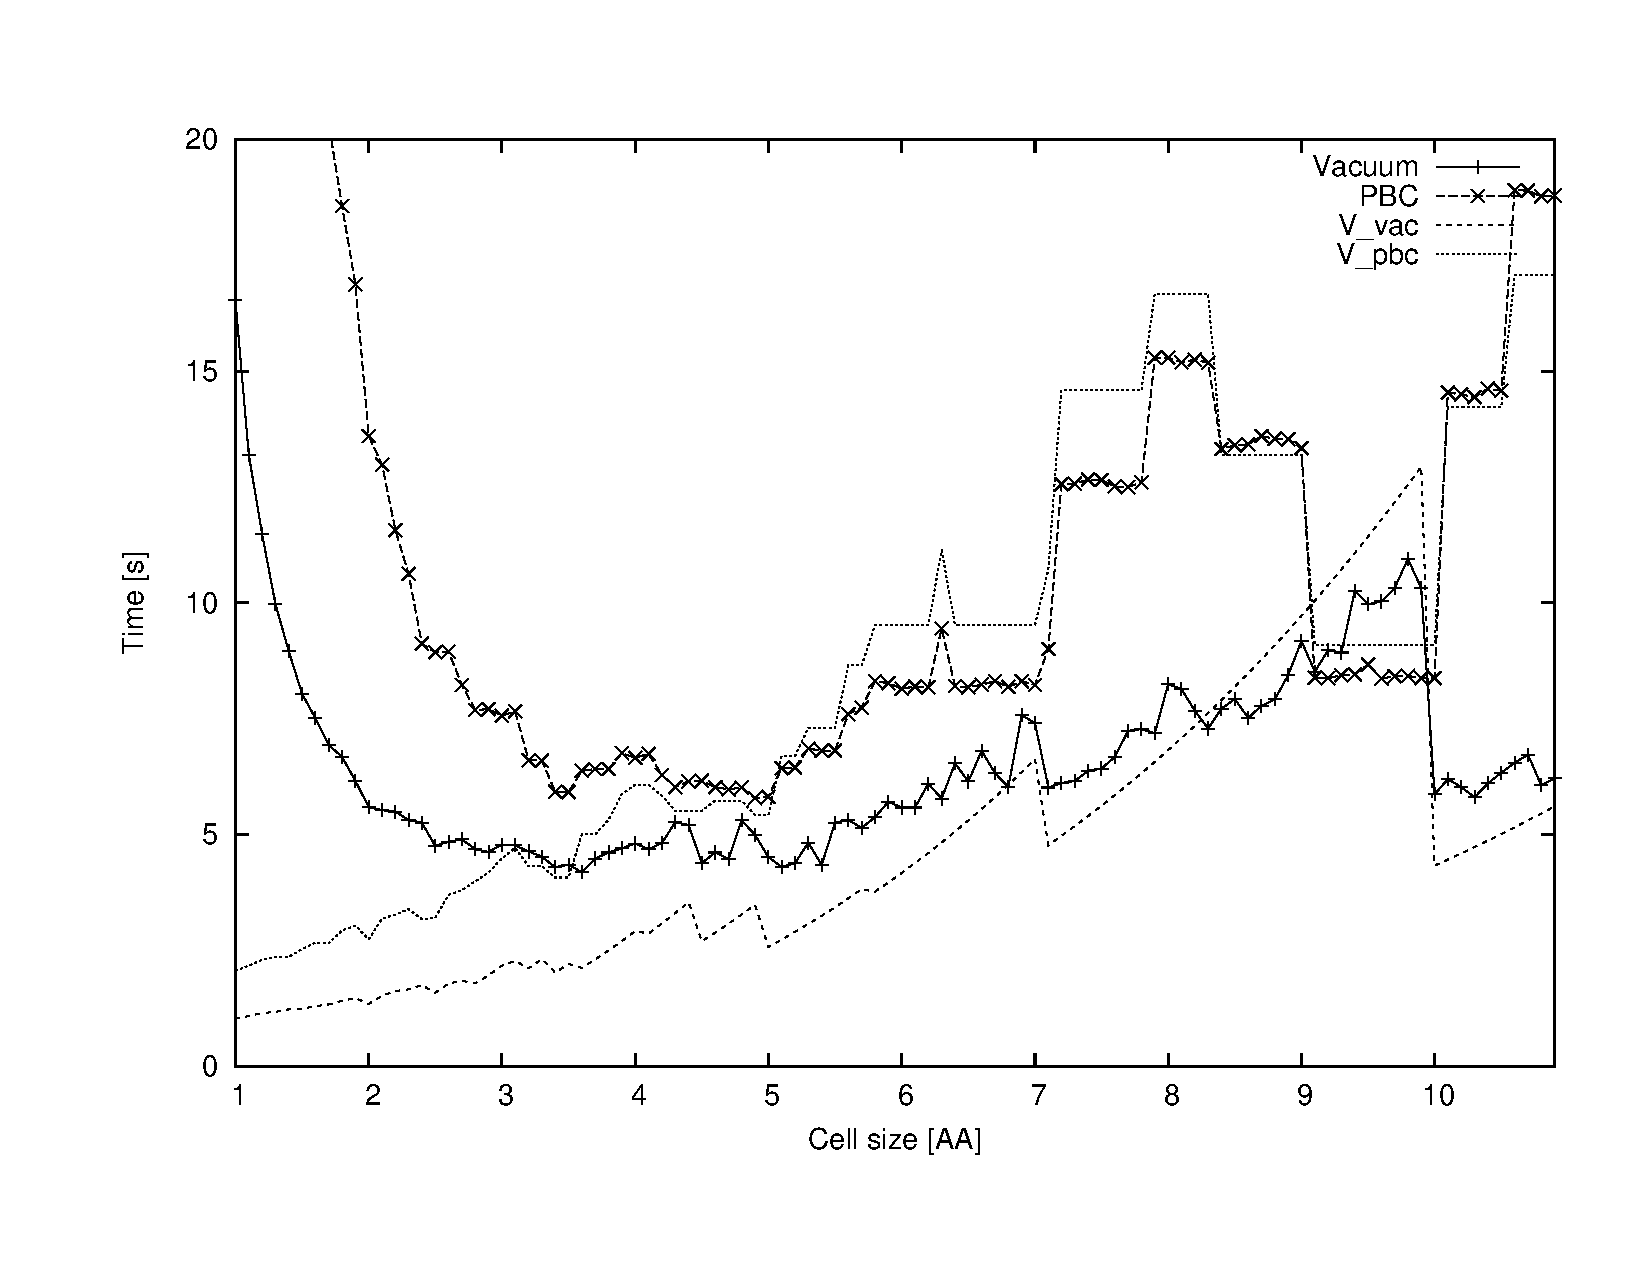
\includegraphics[width=13cm]{cellsize.pdf}}}
\caption{BPTI 14281 Atoms, run with different cell sizes, vacuum and
  PBC, cutoff 10[\AA].}
\label{fig:cellsize}
\end{figure}
which are equal or less distant than the actual cutoff. A cell size
bigger than the cutoff will result with more pairs which are more
distant than the cutoff, where a smaller cell size will increase the
total number of cells to cover the system, decrease the number of particles per cell and 
make the retrieval of candidates more accurate.
The cutoff methods themself have
a cutoff at which distance particles further away as neglected. The
cutoff methods normally offers different switching function to achieve certain
properties, i.e., $C^2$-continues at the cutoff point. The cell size
should be chosen dependent on the cutoff's of all forces, also
considering those coming from switching functions and fast electrostatic
forces. In case of vacuum, the cell dimensions will be defined exactly the
given cell size, where as for periodic boundary conditions the cell
dimensions are chosen such that the number of cells in the simulation
box is maximal, but with at least dimensions defined by the cell size.
For small periodic systems the actual cell dimensions may be significant
lager than the cell size to fit the system box. Choosing the cell size as
the maximum of all cutoff is for most systems a good starting
point. One may also try out the cell sizes such that the maximal
cutoff is a multiple. The smaller the cell size the less particles
reside in a single cell, and increasing the overhead of the cell list
algorithm. On the other hand, a cell size which is smaller (a
multiple) than the cutoff enables the cell list algorithm to decrease
the domain (volume) to pick pair-wise candidates to
interact. Fig.\ref{fig:cellsize} gives a rough picture how performance
may change with a different cell size. For small cell sizes ($<3$) the
overhead of the cell list is significant, especially for vacuum where
the total number of cells variate more often. The volume to pick
possible candidates is small and close to a sphere. For cell sizes
$>3$ and $<5$ one reaches best performance, especially for cell size
$3\frac{1}{3}$ and $5$. For lager cell sizes ($>5$) the performance
follows more or less the volume curve, but for cell size $10$ the
volumes drops and the performance gets better again.
One can also see that with periodic boundary conditions the performance is more stair
alike due to the fact that the real cell dimensions are always a
multiple of the system dimensions, but at least the cell size. The saw
effect for vacuum is due to constant number of total cells until the
cells a big enough to cover the system with less cells.

\clearpage

\subsection{Fast electrostatic methods}

Three main fast electrostatic force mtheods are supported:
\begin{itemize}
\item Ewald, $O(N^{\frac{3}{2}})$
\item Particle-Mesh-Ewald, $O(N\log(N))$
\item Multi Grid, $O(N)$
\end{itemize}

Please consult their tutorials.

% # cellsize pbc        cells       delta  V_cell           V_delat      npc       cells    delta  V_cell           V_delta
% 1.0        79.24440   157500	  6204 	 157500 	  6204	       16.52883  148862   3102 	 148862 	  3102	       
% 1.1        59.97576   115425	  4788 	 157500 	  6533.33      13.19907  108416   2460 	 144302 	  3274.26      
% 1.2        47.85662   87412 	  3838 	 157500 	  6915.35      11.48919  87412 	  2003 	 151048 	  3461.18      
% 1.3        38.76726   69312 	  3112 	 157500 	  7071.5       9.97930   69312 	  1616 	 152278 	  3550.35      
% 1.4        31.35778   55125 	  2488 	 157500 	  7108.57      8.95937   53900 	  1352 	 147902 	  3709.89      
% 1.5        27.78804   45738 	  2206 	 157500 	  7596.42      8.03943   44649 	  1111 	 150690 	  3749.62      
% 1.6        24.18829   37479 	  1910 	 157500 	  8026.49      7.50947   37479 	  955 	 153514 	  3911.68      
% 1.7        20.33856   31117 	  1576 	 157500 	  7976.99      6.92951   31117 	  820 	 152878 	  4028.66      
% 1.8        18.55869   25515 	  1428 	 157500 	  8814.81      6.67953   25515 	  730 	 148803 	  4257.36      
% 1.9        16.86881   22308 	  1292 	 157500 	  9121.84      6.15956   22308 	  646 	 153011 	  4430.91      
% 2.0        13.59904   19375 	  1014 	 157500 	  8242.84      5.59961   19375 	  507 	 155000 	  4056	       
% 2.1        12.97908   15870 	  966 	 157500 	  9586.96      5.52961   15870 	  495 	 146972 	  4584.2       
% 2.2        11.56918   13552 	  846 	 157500 	  9832.13      5.49961   13552 	  459 	 144302 	  4887.43      
% 2.3        10.62925   11907 	  770 	 157500 	  10185.2      5.31962   11907 	  411 	 144872 	  5000.64      
% 2.4        9.11935    10400 	  630 	 157500 	  9540.87      5.25963   11466 	  381 	 158506 	  5266.94      
% 2.5        8.93937    10000 	  612 	 157500 	  9639	       4.75966   10000 	  306 	 156250 	  4781.25      
% 2.6        8.94937    8664 	  612 	 157500 	  11125.3      4.84966   8664 	  306 	 152278 	  5378.26      
% 2.7        8.22942    7452 	  540 	 157500 	  11413	       4.89965   7452 	  282 	 146678 	  5550.61      
% 2.8        7.68946    6358 	  484 	 157500 	  11989.6      4.68967   7128 	  246 	 156474 	  5400.19      
% 2.9        7.70946    6069 	  484 	 157500 	  12560.6      4.62967   6358 	  242 	 155065 	  5902.14      
% 3.0        7.56947    5376 	  460 	 157500 	  13476.6      4.78966   6069 	  242 	 163863 	  6534	       
% 3.1        7.65946    5120 	  460 	 157500 	  14150.4      4.76966   5120 	  230 	 152530 	  6851.93      
% 3.2        6.60953    4275 	  352 	 157500 	  12968.4      4.63967   5120 	  194 	 167772 	  6356.99      
% 3.3        6.59953    4275 	  352 	 157500 	  12968.4      4.52968   4275 	  194 	 153631 	  6971.78      
% 3.4        5.92958    3528 	  274 	 157500 	  12232.1      4.29970   4275 	  155 	 168025 	  6092.12      
% 3.5        5.91958    3528 	  274 	 157500 	  12232.1      4.35969   3528 	  155 	 151263 	  6645.62      
% 3.6        6.37955    2873 	  274 	 157500 	  15020.9      4.18970   3528 	  137 	 164602 	  6391.87      
% 3.7        6.41955    2873 	  274 	 157500 	  15020.9      4.48968   3332 	  137 	 168776 	  6939.46      
% 3.8        6.41955    2704 	  274 	 157500 	  15959.7      4.61967   2873 	  137 	 157647 	  7517.46      
% 3.9        6.75952    2304 	  258 	 157500 	  17636.7      4.70967   2704 	  137 	 160399 	  8126.7       
% 4.0        6.65953    2160 	  250 	 157500 	  18229.2      4.80966   2704 	  137 	 173056 	  8768	       
% 4.1        6.74952    2160 	  250 	 157500 	  18229.2      4.68967   2160 	  125 	 148869 	  8615.12      
% 4.2        6.28956    1815 	  202 	 157500 	  17528.9      4.81966   2160 	  125 	 160030 	  9261	       
% 4.3        6.02957    1694 	  178 	 157500 	  16549.6      5.26963   2160 	  125 	 171735 	  9938.38      
% 4.4        6.14956    1694 	  178 	 157500 	  16549.6      5.20963   1694 	  125 	 144302 	  10648	       
% 4.5        6.16956    1694 	  178 	 157500 	  16549.6      4.38969   1694 	  89 	 154366 	  8110.12      
% 4.6        6.02957    1300 	  142 	 157500 	  17203.8      4.61967   1694 	  89 	 164887 	  8662.9       
% 4.7        5.97958    1300 	  142 	 157500 	  17203.8      4.47968   1694 	  89 	 175876 	  9240.25      
% 4.8        6.01957    1300 	  142 	 157500 	  17203.8      5.30962   1573 	  89 	 173961 	  9842.69      
% 4.9        5.78959    1200 	  124 	 157500 	  16275	       4.99965   1300 	  89 	 152944 	  10470.8      
% 5.0        5.81959    1200 	  124 	 157500 	  16275	       4.51968   1300 	  62 	 162500 	  7750	       
% 5.1        6.43954    972 	  124 	 157500 	  20092.6      4.30970   1300 	  62 	 172446 	  8224.36      
% 5.2        6.44954    972 	  124 	 157500 	  20092.6      4.38969   1200 	  62 	 168730 	  8717.7       
% 5.3        6.85951    891 	  124 	 157500 	  21919.2      4.82966   1200 	  62 	 178652 	  9230.37      
% 5.4        6.80952    891 	  124 	 157500 	  21919.2      4.34969   972 	  62 	 153055 	  9762.77      
% 5.5        6.81952    891 	  124 	 157500 	  21919.2      5.25963   972 	  62 	 161716 	  10315.2        
% 5.6        7.59946    704 	  116 	 157500 	  25951.7      5.31962   891 	  62 	 156474 	  10888.2      
% 5.7        7.73945    704 	  116 	 157500 	  25951.7      5.14964   891 	  62 	 165007 	  11482	       
% 5.8        8.30941    640 	  116 	 157500 	  28546.9      5.37962   891 	  58 	 173845 	  11316.5      
% 5.9        8.26941    640 	  116 	 157500 	  28546.9      5.70960   891 	  58 	 182993 	  11912	       
% 6.0        8.14942    640 	  116 	 157500 	  28546.9      5.58961   891 	  58 	 192456 	  12528	       
% 6.1        8.19942    640 	  116 	 157500 	  28546.9      5.58960   704 	  58 	 159795 	  13164.9      
% 6.2        8.17942    640 	  116 	 157500 	  28546.9      6.09957   640 	  58 	 152530 	  13823	       
% 6.3        9.44933    490 	  104 	 157500 	  33428.6      5.77959   640 	  58 	 160030 	  14502.7      
% 6.4        8.20942    441 	  80 	 157500 	  28571.4      6.53954   640 	  58 	 167772 	  15204.4      
% 6.5        8.17942    441 	  80 	 157500 	  28571.4      6.14957   640 	  58 	 175760 	  15928.2      
% 6.6        8.23942    441 	  80 	 157500 	  28571.4      6.80952   640 	  58 	 183997 	  16674.8      
% 6.7        8.30941    441 	  80 	 157500 	  28571.4      6.32955   640 	  58 	 192488 	  17444.3      
% 6.8        8.18942    441 	  80 	 157500 	  28571.4      6.02957   640 	  58 	 201236 	  18237.1      
% 6.9        8.30941    441 	  80 	 157500 	  28571.4      7.57946   441 	  58 	 144872 	  19053.5      
% 7.0        8.22942    441 	  80 	 157500 	  28571.4      7.40948   441 	  58 	 151263 	  19894	       
% 7.1        9.00936    392 	  80 	 157500 	  32142.9      6.01957   441 	  40 	 157839 	  14316.4      
% 7.2        12.55911   288 	  80 	 157500 	  43750	       6.11957   441 	  40 	 164602 	  14929.9      
% 7.3        12.56911   288 	  80 	 157500 	  43750	       6.15956   441 	  40 	 171556 	  15560.7      
% 7.4        12.65910   288 	  80 	 157500 	  43750	       6.37955   441 	  40 	 178704 	  16209	       
% 7.5        12.64911   288 	  80 	 157500 	  43750	       6.42955   441 	  40 	 186047 	  16875	       
% 7.6        12.50911   288 	  80 	 157500 	  43750	       6.67953   441 	  40 	 193588 	  17559	       
% 7.7        12.49912   288 	  80 	 157500 	  43750	       7.23949   392 	  40 	 178961 	  18261.3      
% 7.8        12.59911   288 	  80 	 157500 	  43750	       7.27949   392 	  40 	 186024 	  18982.1      
% 7.9        15.28892   252 	  80 	 157500 	  50000	       7.18949   392 	  40 	 193271 	  19721.6      
% 8.0        15.28892   252 	  80 	 157500 	  50000	       8.24942   392 	  40 	 200704 	  20480	       
% 8.1        15.18893   252 	  80 	 157500 	  50000	       8.13943   288 	  40 	 153055 	  21257.6      
% 8.2        15.24892   252 	  80 	 157500 	  50000	       7.67946   288 	  40 	 158794 	  22054.7      
% 8.3        15.17893   252 	  80 	 157500 	  50000	       7.28949   288 	  40 	 164675 	  22871.5      
% 8.4        13.31906   175 	  44 	 157500 	  39600	       7.71946   288 	  40 	 170699 	  23708.2      
% 8.5        13.39905   175 	  44 	 157500 	  39600	       7.92944   288 	  40 	 176868 	  24565	       
% 8.6        13.41905   175 	  44 	 157500 	  39600	       7.51947   288 	  40 	 183184 	  25442.2      
% 8.7        13.59904   175 	  44 	 157500 	  39600	       7.77945   288 	  40 	 189649 	  26340.1      
% 8.8        13.53904   175 	  44 	 157500 	  39600	       7.91944   252 	  40 	 171731 	  27258.9      
% 8.9        13.52904   175 	  44 	 157500 	  39600	       8.43941   252 	  40 	 177652 	  28198.8      
% 9.0        13.33906   175 	  44 	 157500 	  39600	       9.17935   252 	  40 	 183708 	  29160	       
% 9.1        8.38941    150 	  26 	 157500 	  27300	       8.51940   252 	  40 	 189900 	  30142.8      
% 9.2        8.37941    150 	  26 	 157500 	  27300	       8.97937   252 	  40 	 196229 	  31147.5      
% 9.3        8.43940    150 	  26 	 157500 	  27300	       8.92937   252 	  40 	 202698 	  32174.3      
% 9.4        8.45940    150 	  26 	 157500 	  27300	       10.25928  252 	  40 	 209307 	  33223.4      
% 9.5        8.66939    150 	  26 	 157500 	  27300	       9.96930   252 	  40 	 216058 	  34295	       
% 9.6        8.36941    150 	  26 	 157500 	  27300	       10.02929  252 	  40 	 222953 	  35389.4      
% 9.7        8.41941    150 	  26 	 157500 	  27300	       10.31927  175 	  40 	 159718 	  36506.9      
% 9.8        8.42941    150 	  26 	 157500 	  27300	       10.94923  175 	  40 	 164709 	  37647.7      
% 9.9        8.37941    150 	  26 	 157500 	  27300	       10.31927  175 	  40 	 169802 	  38812	       
% 10.0       8.37941    150 	  26 	 157500 	  27300	       5.86959   175 	  13 	 175000 	  13000	       
% 10.1       14.53897   96 	  26 	 157500 	  42656.2      6.19956   175 	  13 	 180303 	  13393.9      
% 10.2       14.49898   96 	  26 	 157500 	  42656.2      6.02958   175 	  13 	 185711 	  13795.7      
% 10.3       14.43898   96 	  26 	 157500 	  42656.2      5.80959   150 	  13 	 163909 	  14205.5      
% 10.4       14.61897   96 	  26 	 157500 	  42656.2      6.10957   150 	  13 	 168730 	  14623.2      
% 10.5       14.57897   96 	  26 	 157500 	  42656.2      6.33955   150 	  13 	 173644 	  15049.1      
% 10.6       18.89867   80 	  26 	 157500 	  51187.5      6.54954   150 	  13 	 178652 	  15483.2      
% 10.7       18.88867   80 	  26 	 157500 	  51187.5      6.72953   150 	  13 	 183756 	  15925.6      
% 10.8       18.76868   80 	  26 	 157500 	  51187.5      6.06957   150 	  13 	 188957 	  16376.3      
% 10.9       18.78867   80 	  26 	 157500 	  51187.5      6.21956   150 	  13 	 194254 	  16835.4      

\subsubsection{Evaluation of two potentials simultaneously}

One on the simples and most effective performance tuning is to combine two
potentials evaluated by a cutoff or direct method. {\sc ProtoMol} offers 
to combine the pair-wise potentials to be compute at the same time, which for big
systems convergences to a improvement of close to 2. This idea does also
apply for the fast electrostatic forces, which have a pair-wise
part. For the exmaple BPTI with 14281 atoms the total force evaluatation
takes 9.1s for 10 steps:
\begin{verbatim}
    Force LennardJones 
      -switchingFunction C2 
      -algorithm NonbondedCutoff
      -switchon 1        # C2 swf switch on
      -cutoff 8          # C2 swf cutoff
      -cutoff 8          # algorithm cutoff
    Force Coulomb 
      -switchingFunction Shift 
      -algorithm NonbondedCutoff
      -cutoff 10         # shift swf cutoff
      -cutoff 10         # algorithm cutoff
\end{verbatim}
Where combinding reduces the total force evaluation to 5.8s:
\begin{verbatim}
    Force LennardJones Coulomb 
      -switchingFunction C2 
      -switchingFunction Shift 
      -algorithm NonbondedCutoff
      -switchon 1        # C2 swf switch on
      -cutoff 8          # C2 swf cutoff
      -cutoff 10         # shift swf cutoff
      -cutoff 10         # algorithm cutoff
\end{verbatim}

\subsubsection{Look-up tables}

One may also consider to replace computational expensive pair-wise
potentials by look-up tables, but at a price of more memory
consumption, lower accuracy and increase of cache misses. 

\end{document}
 